\documentclass[11pt,a4paper]{report}
\usepackage[textwidth=37em,vmargin=30mm]{geometry}
\usepackage{calc,xunicode,amsmath,amssymb,paralist,enumitem,tabu,booktabs,datetime2,xeCJK,xeCJKfntef,listings}
\usepackage{tocloft,fancyhdr,tcolorbox,xcolor,graphicx,eso-pic,xltxtra,xelatexemoji}

\newcommand{\envyear}[0]{2024}
\newcommand{\envdatestr}[0]{2024-10-20}
\newcommand{\envfinaldir}[0]{webdb/2024/20241020/final}

\usepackage[hidelinks]{hyperref}
\hypersetup{
    colorlinks=false,
    pdfpagemode=FullScreen,
    pdftitle={Web Digest - \envdatestr}
}

\setlength{\cftbeforechapskip}{10pt}
\renewcommand{\cftchapfont}{\rmfamily\bfseries\large\raggedright}
\setlength{\cftbeforesecskip}{2pt}
\renewcommand{\cftsecfont}{\sffamily\small\raggedright}

\setdefaultleftmargin{2em}{2em}{1em}{1em}{1em}{1em}

\usepackage{xeCJK,xeCJKfntef}
\xeCJKsetup{PunctStyle=plain,RubberPunctSkip=false,CJKglue=\strut\hskip 0pt plus 0.1em minus 0.05em,CJKecglue=\strut\hskip 0.22em plus 0.2em}
\XeTeXlinebreaklocale "zh"
\XeTeXlinebreakskip = 0pt


\setmainfont{Brygada 1918}
\setromanfont{Brygada 1918}
\setsansfont{IBM Plex Sans}
\setmonofont{JetBrains Mono NL}
\setCJKmainfont{Noto Serif CJK SC}
\setCJKromanfont{Noto Serif CJK SC}
\setCJKsansfont{Noto Sans CJK SC}
\setCJKmonofont{Noto Sans CJK SC}

\setlength{\parindent}{0pt}
\setlength{\parskip}{8pt}
\linespread{1.15}

\lstset{
	basicstyle=\ttfamily\footnotesize,
	numbersep=5pt,
	backgroundcolor=\color{black!5},
	showspaces=false,
	showstringspaces=false,
	showtabs=false,
	tabsize=2,
	captionpos=b,
	breaklines=true,
	breakatwhitespace=true,
	breakautoindent=true,
	linewidth=\textwidth
}






\newcommand{\coverpic}[2]{
    % argv: itemurl, authorname
    Cover photo by #2~~(\href{#1}{#1})
}
\newcommand{\makeheader}[0]{
    \begin{titlepage}
        % \newgeometry{hmargin=15mm,tmargin=21mm,bmargin=12mm}
        \begin{center}
            
            \rmfamily\scshape
            \fontspec{BaskervilleF}
            \fontspec{Old Standard}
            \fontsize{59pt}{70pt}\selectfont
            WEB\hfill DIGEST
            
            \vfill
            % \vskip 30pt
            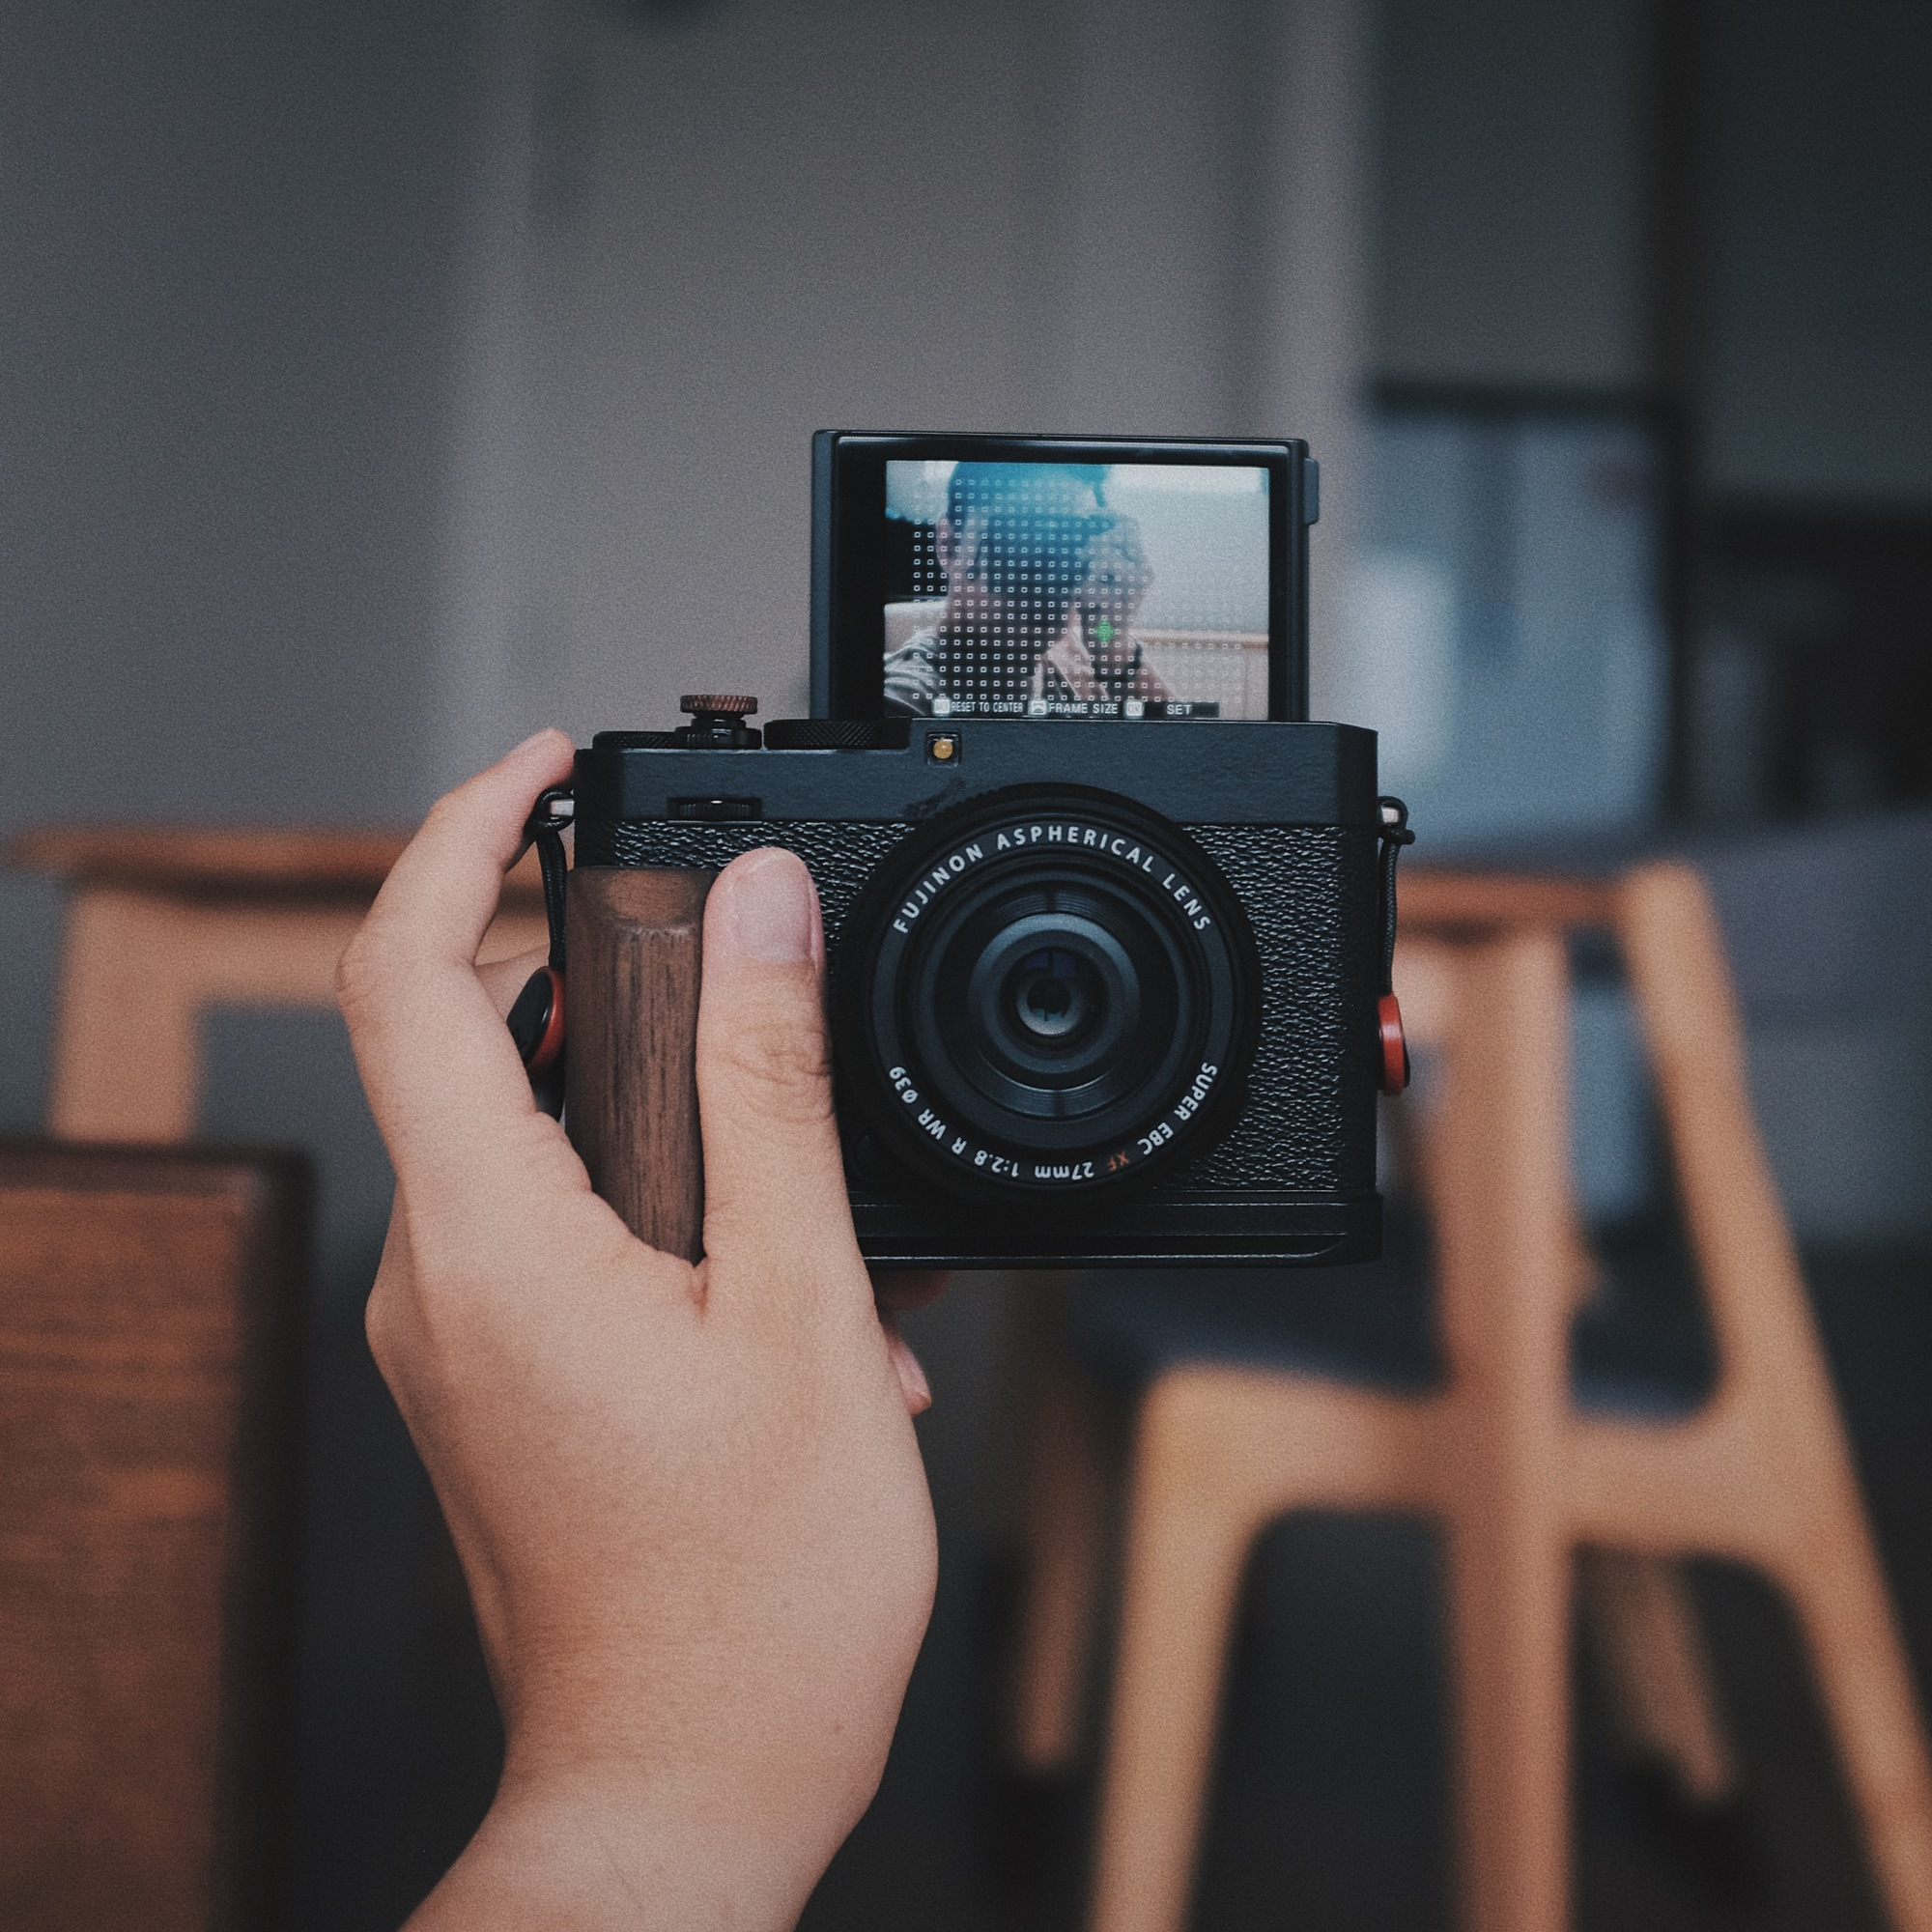
\includegraphics[width=\linewidth]{\envfinaldir/coverpic-prod.jpg}\par
            % \vskip 30pt
            \vfill

            \normalsize\rmfamily\scshape
            \copyright{} The Web Digest Project \hfill\large \envdatestr
        \end{center}
    \end{titlepage}
    % \restoregeometry
}
\newcommand{\simplehref}[1]{%
    \textcolor{blue!80!green}{\href{#1}{#1}}%
}
\renewcommand{\contentsname}{\center\Huge\sffamily\bfseries Contents\par\vskip 20pt}
\newcounter{ipartcounter}
\setcounter{ipartcounter}{0}
\newcommand{\ipart}[1]{
    % \vskip 20pt
    \clearpage
    \stepcounter{ipartcounter}
    \phantomsection
    \addcontentsline{toc}{chapter}{#1}
    % \begin{center}
    %     \Huge
    %     \sffamily\bfseries
    %     #1
    % \end{center}
    % \vskip 20pt plus 7pt
}
\newcounter{ichaptercounter}
\setcounter{ichaptercounter}{0}
\newcommand{\ichapter}[1]{
    % \vskip 20pt
    \clearpage
    \stepcounter{ichaptercounter}
    \phantomsection
    \addcontentsline{toc}{section}{\numberline{\arabic{ichaptercounter}}#1}
    \begin{center}
        \Huge
        \sffamily\bfseries
        #1
    \end{center}
    \vskip 20pt plus 7pt
}
\newcommand{\entrytitlefont}[1]{\subsection*{\raggedright\Large\sffamily\bfseries#1}}
\newcommand{\entryitemGeneric}[2]{
    % argv: title, url
    \parbox{\linewidth}{
        \entrytitlefont{#1}\par\vskip 5pt
        \footnotesize\ttfamily\mdseries
        \simplehref{#2}
    }\vskip 11pt plus 11pt minus 1pt
}
\newcommand{\entryitemGithub}[3]{
    % argv: title, url, desc
    \parbox{\linewidth}{
        \entrytitlefont{#1}\par\vskip 5pt
        \footnotesize\ttfamily\mdseries
        \simplehref{#2}\par\vskip 5pt
        \small\rmfamily\mdseries#3
    }\vskip 11pt plus 11pt minus 1pt
}
\newcommand{\entryitemAp}[3]{
    % argv: title, url, desc
    \parbox{\linewidth}{
        \entrytitlefont{#1}\par\vskip 5pt
        \footnotesize\ttfamily\mdseries
        \simplehref{#2}\par\vskip 5pt
        \small\rmfamily\mdseries#3
    }\vskip 11pt plus 11pt minus 1pt
}
\newcommand{\entryitemHackernews}[3]{
    % argv: title, hnurl, rawurl
    % \parbox{\linewidth}{
    %     \entrytitlefont{#1}\par\vskip 5pt
    %     \footnotesize\ttfamily\mdseries
    %     \simplehref{#3}\par
    %     \textcolor{black!50}{\href{#2}{#2}}
    % }\vskip 11pt plus 11pt minus 1pt
    \begin{minipage}{\linewidth}
            \entrytitlefont{#1}\par\vskip 5pt
            \footnotesize\ttfamily\mdseries
            \simplehref{#3}\par
            \textcolor{black!50}{\href{#2}{#2}}
    \end{minipage}\par\vskip 11pt plus 11pt minus 1pt
}







\begin{document}

\makeheader

\tableofcontents\clearpage




\ipart{Developers}
\ichapter{Hacker News}
\entryitemTwoLinks{QUIC Is Not Quick Enough over Fast Internet}{https://news.ycombinator.com/item?id=41890784}{https://arxiv.org/abs/2310.09423}

\entryitemTwoLinks{Svelte 5 Released}{https://news.ycombinator.com/item?id=41889674}{https://www.npmjs.com/package/svelte}

\entryitemTwoLinks{Dwarf Fortress – Boatmurdered Part \#1 – Intro (2006)}{https://news.ycombinator.com/item?id=41889543}{https://lparchive.org/Dwarf-Fortress-Boatmurdered/Introduction/}

\entryitemTwoLinks{AI engineers claim new algorithm reduces AI power consumption by 95\%}{https://news.ycombinator.com/item?id=41889414}{https://www.tomshardware.com/tech-industry/artificial-intelligence/ai-engineers-build-new-algorithm-for-ai-processing-replace-complex-floating-point-multiplication-with-integer-addition}

\entryitemTwoLinks{Love being interrupted when my monitor asks me to accept user agreements}{https://news.ycombinator.com/item?id=41889140}{https://twitter.com/snwy\_me/status/1847396175961641176}

\entryitemTwoLinks{A Distributed Systems Reading List (2014)}{https://news.ycombinator.com/item?id=41889076}{https://dancres.github.io/Pages/}

\entryitemTwoLinks{Have McKinsey and its consulting rivals got too big?}{https://news.ycombinator.com/item?id=41888061}{https://www.economist.com/business/2024/03/25/have-mckinsey-and-its-consulting-rivals-got-too-big}

\entryitemTwoLinks{Send: Open-source fork of Firefox Send}{https://news.ycombinator.com/item?id=41887378}{https://send.vis.ee/}

\entryitemTwoLinks{S3 as a Git remote and LFS server}{https://news.ycombinator.com/item?id=41887004}{https://github.com/awslabs/git-remote-s3}

\entryitemTwoLinks{The long road to lazy preemption in the Linux CPU scheduler}{https://news.ycombinator.com/item?id=41886256}{https://lwn.net/SubscriberLink/994322/45aa5211a50bc63a/}

\entryitemTwoLinks{How to leverage Claude's capabilities with interactive visualization}{https://news.ycombinator.com/item?id=41885231}{https://github.com/anthropics/anthropic-quickstarts/tree/main/financial-data-analyst}

\entryitemTwoLinks{US probes Tesla's Full Self-Driving software in 2.4M cars after fatal crash}{https://news.ycombinator.com/item?id=41884740}{https://www.reuters.com/business/autos-transportation/nhtsa-opens-probe-into-24-mln-tesla-vehicles-over-full-self-driving-collisions-2024-10-18/}

\entryitemTwoLinks{Express v5}{https://news.ycombinator.com/item?id=41882955}{https://expressjs.com/2024/10/15/v5-release.html}

\entryitemTwoLinks{Focus on decisions, not tasks}{https://news.ycombinator.com/item?id=41881872}{https://technicalwriting.dev/strategy/decisions.html}

\entryitemTwoLinks{The feds are coming for John Deere over the right to repair}{https://news.ycombinator.com/item?id=41880981}{https://gizmodo.com/the-feds-are-coming-for-john-deere-over-the-right-to-repair-2000513521}

\entryitemTwoLinks{Subvert – Collectively owned music marketplace}{https://news.ycombinator.com/item?id=41880829}{https://subvert.fm/}

\entryitemTwoLinks{US probes Tesla's Full Self-Driving software after fatal crash}{https://news.ycombinator.com/item?id=41880649}{https://www.reuters.com/business/autos-transportation/nhtsa-opens-probe-into-24-mln-tesla-vehicles-over-full-self-driving-collisions-2024-10-18/}

\entryitemTwoLinks{Show HN: Go Plan9 Memo}{https://news.ycombinator.com/item?id=41879854}{https://pehringer.info/go\_plan9\_memo.html}

\entryitemTwoLinks{Running an open source app: Usage, costs and community donations}{https://news.ycombinator.com/item?id=41879845}{https://spliit.app/blog/spliit-by-the-stats-usage-costs-donations}

\entryitemTwoLinks{Code that helped end Apartheid}{https://news.ycombinator.com/item?id=41879072}{https://www.wired.com/story/plaintext-you-can-now-see-the-code-that-ended-apartheid/}\ichapter{Phoronix}
\entryitemGeneric{\hskip 0pt{}"100\% Free" GNU Boot Discovers Again They Have Been Shipping Non-Free Code}{https://www.phoronix.com/news/GNU-Boot-Second-Fail}

\entryitemGeneric{\hskip 0pt{}GNOME Making Progress On Full-Featured USB Portal For Flatpaks}{https://www.phoronix.com/news/GNOME-USB-Flatpaks-Portal}

\entryitemGeneric{\hskip 0pt{}Wine-Staging 9.20 Fixes An 11 Year Old Wine Bug Report}{https://www.phoronix.com/news/Wine-Staging-9.20}

\entryitemGeneric{\hskip 0pt{}Linux Might Drop Fieldbus Support For Industrial Systems With No One Maintaining It}{https://www.phoronix.com/news/Linux-Might-Drop-Fieldbus}

\entryitemGeneric{\hskip 0pt{}Linux 6.12-rc4 Adding Controller Support For The MSI Claw A1M \& 8BitDo Ultimate 2C}{https://www.phoronix.com/news/Linux-6.12-rc4-MSI-Claw-A1M}

\entryitemGeneric{\hskip 0pt{}KDE Developers Wrapping Up Fallout From Plasma 6.2, Spinning More Plasma 6.3 Features}{https://www.phoronix.com/news/KDE-Plasma-6.2-Bugs-Fixed}

\entryitemGeneric{\hskip 0pt{}Intel Working On Coreboot Support For Xeon 6 Platforms}{https://www.phoronix.com/news/Intel-Xeon-6-Coreboot-Effort}

\entryitemGeneric{\hskip 0pt{}Wine 9.20 Released With WineDbg Now Using Capstone Disassembler}{https://www.phoronix.com/news/Wine-9.20-Released}

\entryitemGeneric{\hskip 0pt{}Ubuntu Considers Replacing initramfs-tools With Dracut}{https://www.phoronix.com/news/Ubuntu-Considers-Dracut-Initrd}


\ipart{Developers~~~~(zh-Hans)}
\ichapter{Solidot}
\entryitemGeneric{\hskip 0pt{}OpenAI 相对于其它 AI 公司的优势基本消失}{https://www.solidot.org/story?sid=79537}

\entryitemGeneric{\hskip 0pt{}古巴电网故障导致千万人断电}{https://www.solidot.org/story?sid=79536}

\entryitemGeneric{\hskip 0pt{}美国越来越多的父母拒绝给孩子接种疫苗}{https://www.solidot.org/story?sid=79535}

\entryitemGeneric{\hskip 0pt{}亚马逊高管告诉员工如果不喜欢强制重返办公室政策他们可以辞职}{https://www.solidot.org/story?sid=79534}

\entryitemGeneric{\hskip 0pt{}人类的嗅觉反应十分迅速}{https://www.solidot.org/story?sid=79533}

\entryitemGeneric{\hskip 0pt{}OpenAI 和微软的紧密关系出现裂缝}{https://www.solidot.org/story?sid=79532}

\entryitemGeneric{\hskip 0pt{}Gliese 229 B 被发现是一对棕矮星}{https://www.solidot.org/story?sid=79531}

\entryitemGeneric{\hskip 0pt{}高中生因使用 AI 受罚,其父母随后起诉教师和校长}{https://www.solidot.org/story?sid=79530}

\entryitemGeneric{\hskip 0pt{}新疗法能消除 2 型糖尿病患者对胰岛素的需求}{https://www.solidot.org/story?sid=79529}

\entryitemGeneric{\hskip 0pt{}欧盟考虑将马斯克其他公司的收入纳入 X 的潜在罚款计算内}{https://www.solidot.org/story?sid=79528}

\entryitemGeneric{\hskip 0pt{}NASA 冻结波音 Starliner 任务}{https://www.solidot.org/story?sid=79527}

\entryitemGeneric{\hskip 0pt{}香港诈骗集团用 AI 深度伪造欺骗受害者}{https://www.solidot.org/story?sid=79526}

\entryitemGeneric{\hskip 0pt{}Meta 解雇了 20 多名用餐券购买家庭用品的员工}{https://www.solidot.org/story?sid=79525}

\entryitemGeneric{\hskip 0pt{}养殖鱼比野生捕捞更不可持续}{https://www.solidot.org/story?sid=79524}

\entryitemGeneric{\hskip 0pt{}Telegram 有数百万用户利用 AI 制作深度伪造色情}{https://www.solidot.org/story?sid=79523}

\entryitemGeneric{\hskip 0pt{}美国起诉了两名 Anonymous Sudan 成员}{https://www.solidot.org/story?sid=79522}

\entryitemGeneric{\hskip 0pt{}保持互联网运行的深海紧急任务}{https://www.solidot.org/story?sid=79521}

\entryitemGeneric{\hskip 0pt{}Matt Mullenweg 的报复行动冲击 WordPress 社区}{https://www.solidot.org/story?sid=79520}

\entryitemGeneric{\hskip 0pt{}哈勃发现木星大红斑大小会变化}{https://www.solidot.org/story?sid=79519}

\entryitemGeneric{\hskip 0pt{}官方机构指责英特尔产品存在网络安全问题}{https://www.solidot.org/story?sid=79518}\ichapter{V2EX}
\entryitemGeneric{\hskip 0pt{}[互联网] 国庆以来,感觉长城又垒高了不少}{https://www.v2ex.com/t/1081839}

\entryitemGeneric{\hskip 0pt{}[问与答] 公司内网,浏览网页的内容可以被监测到吗}{https://www.v2ex.com/t/1081838}

\entryitemGeneric{\hskip 0pt{}[推广] tiktok 上面关于 star of jacob 的讨论你们怎么看 https://starofjacob.org/}{https://www.v2ex.com/t/1081837}

\entryitemGeneric{\hskip 0pt{}[问与答] 现在的即热饮水机 是不是普遍虚假宣传 出水温度不够}{https://www.v2ex.com/t/1081836}

\entryitemGeneric{\hskip 0pt{}[Amazon] 美亚打算买个谷歌手机直邮国内}{https://www.v2ex.com/t/1081835}

\entryitemGeneric{\hskip 0pt{}[问与答] 有人知道这是什么播客软件吗}{https://www.v2ex.com/t/1081834}

\entryitemGeneric{\hskip 0pt{}[问与答] 有什么好用的工具可以在线 提取 抖音视频字幕吗?}{https://www.v2ex.com/t/1081832}

\entryitemGeneric{\hskip 0pt{}[问与答] 谷歌浏览器 chrome 怎么彻底删除书签?}{https://www.v2ex.com/t/1081831}

\entryitemGeneric{\hskip 0pt{}[小米] 请教小米解锁 BL 问题}{https://www.v2ex.com/t/1081830}

\entryitemGeneric{\hskip 0pt{}[职场话题] 判断一份工作的三个指标:工作强度、收入和是否是想做的事}{https://www.v2ex.com/t/1081827}

\entryitemGeneric{\hskip 0pt{}[投资] 用示例解析期权策略 - 保护性看跌期权策略}{https://www.v2ex.com/t/1081826}

\entryitemGeneric{\hskip 0pt{}[Python] 求一份 django4.2 或 django5.x 中文文档 pdf 版 ,谢谢各位}{https://www.v2ex.com/t/1081824}

\entryitemGeneric{\hskip 0pt{}[程序员] vscode 有这种 tcl 插件吗,支持调用的 tcl 函数跳转到定义?}{https://www.v2ex.com/t/1081823}

\entryitemGeneric{\hskip 0pt{}[NAS] 现在还求得到馒头邀请吗?}{https://www.v2ex.com/t/1081822}

\entryitemGeneric{\hskip 0pt{}[Chrome] 请问 chrome 如何设置 DNS over QUIC (DoQ)?}{https://www.v2ex.com/t/1081821}

\entryitemGeneric{\hskip 0pt{}[Chrome] chrome 更新到 130 版本,发现自带``整理标签页''的功能了。}{https://www.v2ex.com/t/1081820}

\entryitemGeneric{\hskip 0pt{}[问与答] 为何 speedtest 中国大陆的节点只剩 11 个了}{https://www.v2ex.com/t/1081819}

\entryitemGeneric{\hskip 0pt{}[分享创造] 后端程序员搞了一个工具小网站, 欢迎来挑刺}{https://www.v2ex.com/t/1081818}

\entryitemGeneric{\hskip 0pt{}[分享创造] 解救你的 40+浏览器标签!一键整理术,让杂乱标签瞬间变精致}{https://www.v2ex.com/t/1081817}

\entryitemGeneric{\hskip 0pt{}[生活] 三十而立:完完全全拥有了自己的第一套房}{https://www.v2ex.com/t/1081814}

\entryitemGeneric{\hskip 0pt{}[问与答] 为什么 MBP 压缩文件效率很慢?}{https://www.v2ex.com/t/1081811}

\entryitemGeneric{\hskip 0pt{}[问与答] 关于 mbp14 的自带的音响}{https://www.v2ex.com/t/1081809}

\entryitemGeneric{\hskip 0pt{}[酷工作] 高级 BlockChain 测试(BTC Layer2 \& DEX -Remote)}{https://www.v2ex.com/t/1081808}

\entryitemGeneric{\hskip 0pt{}[问与答] 如何提高抵抗挫折的能力?}{https://www.v2ex.com/t/1081806}

\entryitemGeneric{\hskip 0pt{}[VPS] 讨论 VPS 上下载的大文件如何优雅地访问/拖回本地}{https://www.v2ex.com/t/1081805}

\entryitemGeneric{\hskip 0pt{}[奇思妙想] Windows 如果开放自定义 UI}{https://www.v2ex.com/t/1081804}

\entryitemGeneric{\hskip 0pt{}[Apple] HomePod 怎么也有 bug 了,一首歌还剩 50 多秒就没有声音了}{https://www.v2ex.com/t/1081802}

\entryitemGeneric{\hskip 0pt{}[问与答] 我现在有一个暴论:如果音视频应用只提供移动端,那么抓包逆向下载的难度会直线上升!}{https://www.v2ex.com/t/1081801}

\entryitemGeneric{\hskip 0pt{}[酷工作] 有个需求,不是要求多高的技术能力.能写 ai promt, 善于沟通, 3 年工作经验. 成都. 销售形式公司.}{https://www.v2ex.com/t/1081799}

\entryitemGeneric{\hskip 0pt{}[买买买] 各位买的 VIVO X200 PRO 是多少钱}{https://www.v2ex.com/t/1081798}

\entryitemGeneric{\hskip 0pt{}[分享创造] IP 查询工具站 UI 更新,新增 ICP 备案查询功能}{https://www.v2ex.com/t/1081797}

\entryitemGeneric{\hskip 0pt{}[分享创造] 《代码时光机》播客第 6 期更新 :)}{https://www.v2ex.com/t/1081796}

\entryitemGeneric{\hskip 0pt{}[VXNA] 申请收录个人博客:通灵卡片 Psychic Paper}{https://www.v2ex.com/t/1081795}

\entryitemGeneric{\hskip 0pt{}[分享发现] 淘宝官方客服骚操作,商品虚假宣传,退货判我出一半运费}{https://www.v2ex.com/t/1081794}

\entryitemGeneric{\hskip 0pt{}[Windows] 谁能举个例子, Win11 究竟哪儿不好用了?}{https://www.v2ex.com/t/1081793}

\entryitemGeneric{\hskip 0pt{}[宽带症候群] 宽带被拉小黑屋,刷外网比内网快}{https://www.v2ex.com/t/1081792}

\entryitemGeneric{\hskip 0pt{}[分享发现] 《纳瓦尔宝典》读书笔记}{https://www.v2ex.com/t/1081791}

\entryitemGeneric{\hskip 0pt{}[分享创造] [网站自荐] 数字华容道游戏 - 挑战玩家的逻辑思维和空间推理能力的免费在线数字推盘益智游戏}{https://www.v2ex.com/t/1081789}

\entryitemGeneric{\hskip 0pt{}[分享发现] 万事达刷北京地铁免单,北京坐地铁通勤的可以关注下。}{https://www.v2ex.com/t/1081788}

\entryitemGeneric{\hskip 0pt{}[OpenWrt] Openwrt wifi 5G 把 channel 从 39 改成 149 , 竟然无线信号好了很多}{https://www.v2ex.com/t/1081787}

\entryitemGeneric{\hskip 0pt{}[路由器] 零刻倍控畅网的 N100 机器哪个好}{https://www.v2ex.com/t/1081786}

\entryitemGeneric{\hskip 0pt{}[求职] 求一份 web3 行业的前端或则全栈工作}{https://www.v2ex.com/t/1081784}

\entryitemGeneric{\hskip 0pt{}[分享创造] [剪贴板工具 WeClipper] Devlog\#02 发布 Alpha 测试版(仅 2.6MB)}{https://www.v2ex.com/t/1081783}

\entryitemGeneric{\hskip 0pt{}[宽带症候群] 遇到一个奇怪的网络问题}{https://www.v2ex.com/t/1081782}

\entryitemGeneric{\hskip 0pt{}[MacBook Pro] 用慢充给 M1 mac 充电。会不会延长电池寿命? 循环次数多但衰减少}{https://www.v2ex.com/t/1081781}

\entryitemGeneric{\hskip 0pt{}[问与答] 送女朋友哪一个比较合适?}{https://www.v2ex.com/t/1081780}

\entryitemGeneric{\hskip 0pt{}[生活] [记录]2024-10-15 VegaFina 1998 52 雪茄品尝}{https://www.v2ex.com/t/1081779}

\entryitemGeneric{\hskip 0pt{}[分享创造] 2024,我们做了一个纯粹的文字社区}{https://www.v2ex.com/t/1081778}

\entryitemGeneric{\hskip 0pt{}[问与答] 广电宽带不支持 ipv6?}{https://www.v2ex.com/t/1081777}

\entryitemGeneric{\hskip 0pt{}[Cloudflare] 设置域名 A 记录 Proxied 后, CF 默认会缓存 css/js 等静态文件吗?}{https://www.v2ex.com/t/1081776}


\ipart{Generic News}
\ichapter{AP News}
\entryitemWithDescription{\hskip 0pt{}9 monkeys die in 2 days under mysterious circumstances at Hong Kong zoo}{https://apnews.com/article/57cb32f0ab09bb5537385f9c6bb145ab}{}\ichapter{Reuters}
\entryitemWithDescription{\hskip 0pt{}Britain's King Charles and Queen Camilla to attend Sydney church on royal tour}{https://www.reuters.com/world/uk/britains-king-charles-queen-camilla-attend-sydney-church-royal-tour-2024-10-19/}{Britain\textquotesingle s King Charles and Queen Camilla will attend a service at St Thomas\textquotesingle{} Anglican church and meet residents in North Sydney on Sunday, as the first day of the official tour program in...}

\entryitemWithDescription{\hskip 0pt{}North Korea foreign minister calls new US-led sanctions monitoring team unlawful, KCNA says}{https://www.reuters.com/world/asia-pacific/north-korea-foreign-minister-calls-new-us-led-sanctions-monitoring-team-unlawful-2024-10-19/}{North Korea\textquotesingle s foreign minister said a new multilateral sanctions monitoring team led by the United States was "utterly unlawful and illegitimate", state media said on...}

\entryitemWithDescription{\hskip 0pt{}Pentagon chief calls on Israel to scale back Beirut strikes}{https://www.reuters.com/world/middle-east/pentagon-chief-calls-israel-scale-back-beirut-strikes-2024-10-19/}{The United States would like to see Israel scale back some of its strikes in and around the Lebanese capital of Beirut, U.S. Defense Secretary Lloyd Austin said on Saturday, adding the number of civilian casualties was "far too...}

\entryitemWithDescription{\hskip 0pt{}Harris says she won't give up pushing for end to Israel-Gaza war}{https://www.reuters.com/world/harris-says-wont-give-up-pushing-end-israel-gaza-war-2024-10-19/}{U.S. Vice President Kamala Harris on Saturday repeated her call for a ceasefire in Israel\textquotesingle s war in Gaza and said it was important to seize the opportunity provided by the killing of Hamas leader Yahya Sinwar, a mastermind...}

\entryitemWithDescription{\hskip 0pt{}Zayn Malik postpones US tour dates after One Direction bandmate Liam Payne's death}{https://www.reuters.com/world/zayn-malik-postpones-us-tour-dates-after-one-direction-bandmate-liam-paynes-2024-10-19/}{British singer Zayn Malik said on Saturday he will postpone the U.S. leg of his "Stairway to the Sky" tour after his former One Direction bandmate Liam Payne died earlier this...}

\entryitemWithDescription{\hskip 0pt{}Hurricane warning issued for Oscar in Bahamas, NHC says}{https://www.reuters.com/world/americas/hurricane-warning-issued-oscar-bahamas-nhc-says-2024-10-19/}{The government of the Bahamas has issued a hurricane warning for Tropical Storm Oscar which formed east of the Turks and Caicos islands, the U.S. National Hurricane Center said on...}

\entryitemWithDescription{\hskip 0pt{}Migrants held in Albania transferred to Italy after court ruling}{https://www.reuters.com/world/europe/migrants-held-albania-transferred-italy-after-court-ruling-2024-10-19/}{The Italian government said it would push ahead with Prime Minister Giorgia Meloni\textquotesingle s flagship project to divert asylum-seekers...}

\entryitemWithDescription{\hskip 0pt{}Tropical Storm Nadine sweeps across Belize, dumps rains on Mexico's Yucatan}{https://www.reuters.com/business/environment/tropical-storm-nadine-sweeps-across-belize-dumps-rains-mexicos-yucatan-2024-10-19/}{Tropical Storm Nadine swirled across Belize on Saturday, bringing heavy rains and strong winds to the Central American nation and the neighboring Yucatan Peninsula to the north in...}

\entryitemWithDescription{\hskip 0pt{}G7 defence ministers back Ukraine's 'irreversible path' to NATO membership}{https://www.reuters.com/world/g7-defence-ministers-back-ukraines-irreversible-path-nato-membership-2024-10-19/}{Defence Ministers of the Group of Seven (G7) major democracies support Ukraine\textquotesingle s "irreversible path to full Euro-Atlantic integration, including NATO membership," they said in a statement on...}

\entryitemWithDescription{\hskip 0pt{}Tropical Storm Nadine makes landfall in Belize, NHC says}{https://www.reuters.com/business/environment/tropical-storm-nadine-expected-make-landfall-belize-nhc-says-2024-10-19/}{Tropical Storm Nadine made landfall in Belize on Saturday, the U.S. National Hurricane Center (NHC...}

\entryitemWithDescription{\hskip 0pt{}Germany says Britain taking lead on possible Eurofighters for Turkey}{https://www.reuters.com/business/aerospace-defense/germany-says-britain-taking-lead-possible-eurofighters-turkey-2024-10-19/}{German Chancellor Olaf Scholz said on Saturday that a project to possibly supply Turkey with Eurofighter jets was an effort being driven by Britain and was in the early...}

\entryitemWithDescription{\hskip 0pt{}Cuba making slow progress re-starting power after second grid collapse}{https://www.reuters.com/world/americas/cubas-electrical-grid-collapses-second-time-entire-country-again-without-power-2024-10-19/}{Cuba\textquotesingle s government blames weeks of worsening blackouts on deteriorating infrastructure, fuel shortages and rising...}

\entryitemWithDescription{\hskip 0pt{}Israel air strike kills 73 Palestinians in northern Gaza, Hamas media office says}{https://www.reuters.com/world/middle-east/israeli-strikes-kill-32-gaza-siege-around-hospitals-tightens-health-officials-2024-10-19/}{Palestinian health officials said telecoms and internet services were down for a second day, hampering rescue...}






\clearpage
\leavevmode\vfill
\footnotesize

Copyright \copyright{} 2023-2024 Neruthes and other contributors.

This document is published with CC BY-NC-ND 4.0 license.

The entries listed in this newsletter may be copyrighted by their respective creators.

This newsletter is generated by the Web Digest project.

The newsletters are also delivered via Telegram channel \CJKunderline{\href{https://t.me/webdigestchannel}{https://t.me/webdigestchannel}}.\\
RSS feed is available at \CJKunderline{\href{https://webdigest.pages.dev/rss.xml}{https://webdigest.pages.dev/rss.xml}}.

This newsletter is available in PDF at
\CJKunderline{\href{https://webdigest.pages.dev/}{https://webdigest.pages.dev/}}.

The source code being used to generate this newsletter is available at\\
\CJKunderline{\href{https://github.com/neruthes/webdigest}{https://github.com/neruthes/webdigest}}.

This newsletter is also available in
\CJKunderline{\href{http://webdigest.pages.dev/readhtml/\envyear/WebDigest-20241020.html}{HTML}} and
\CJKunderline{\href{https://github.com/neruthes/webdigest/blob/master/markdown/\envyear/WebDigest-20241020.md}{Markdown}}.


\coverpic{https://unsplash.com/photos/a-tall-red-building-with-a-tree-in-front-of-it-2no2tRs1ynU}{Andrea De Santis}


\end{document}
